\section{Simulations}\label{sec:simulation}

The ODE (open dynamics engine) library \cite{ode:2008} is used for testing the iterative mass displacement compensation algorithm presented in previous section. The initial position of quadruped hopping robot is shown in Fig \ref{fig:ODESimulations}a. Each leg consists of two spring-damper joints, the first passive connects red and green cylinder and the second, active one, connects the green cylinder with the robot body. The body consists of 4 connected masses indexed as 1 (white), 2 (red), 3 (green) and 4 (blue). The whole robot simulation parameters are shown in \ref{tab:RobotDimensions}.

\begin{table}
\centering
\begin{tabular}{|c|c|}
	\hline
	$Body\: size$ &  $[0.30\: 0.15\: 0.01]m$ \\
	\hline
	$Lower\:leg\:size$ &  $0.05m$ \\
	\hline
	$Upper\:leg\:size$ &  $0.05m$ \\
	\hline
	$Leg\:radius$ &  $0.01m$ \\
	\hline
	$Total\:leg\:mass$ &  $0.15kg$ \\
	\hline
	$Passive\:spring\:constant/damping$ &  $2000N/m, 50Ns/m$ \\
	\hline
	$Active\:spring\:constant/damping$ &  $10000N/m, 30Ns/m$ \\
	\hline
	$Tail\:length$ &  $0.1m$ \\
	\hline
	$Tail\:radius$ &  $0.005m$ \\
	\hline
\end{tabular}
\caption{Robot simulation parameters}\label{tab:RobotDimensions}
\end{table}



The active springs iteratively generates forces (Td=1s) which accelerate the body and produces rotational vector which is recorded during acceleration phase. The used actuated spring force is minimal to produce measurable angular speed and to minimize time to calm the body consequential oscillations. The acceleration phase lasts for about 200ms after which the body calms in 800ms. The initial tail angles are $q_1=0$ and $q_2=0$ as positioned in Fig. \ref{fig:ODESimulations}a.

\begin{table}
	\centering
\begin{tabular}{|c|c|c|c|c|}
	\hline
$Test$ &  $Mass[kg]$ & $Q$  & $\left \| \vec{\omega} \right \|$ & $K_0$\\
	\hline
0   & $[0\: 0\: 1\: 1]$ & $[89.99\: 32.86]$ & 0.0026 & 0.3\\
1   & $[1\: 1\: 0\: 0]$ & $[-89.99\: 32.20]$ & 0.0038 & 0.3\\
2   & $[1\: 1\: 1\: 0]$ & $[-25.43\: 29.15]$ &  0.003 & 0.3\\
3   & $[1\: 1\: 1\: 0]$ & $[-26.02\: 29.05]$ &  0.0025 & 0.6\\
\hline
\end{tabular}
\caption{Testing parameters}\label{tab:Simulations}
\end{table}



\begin{figure}
	\centering
	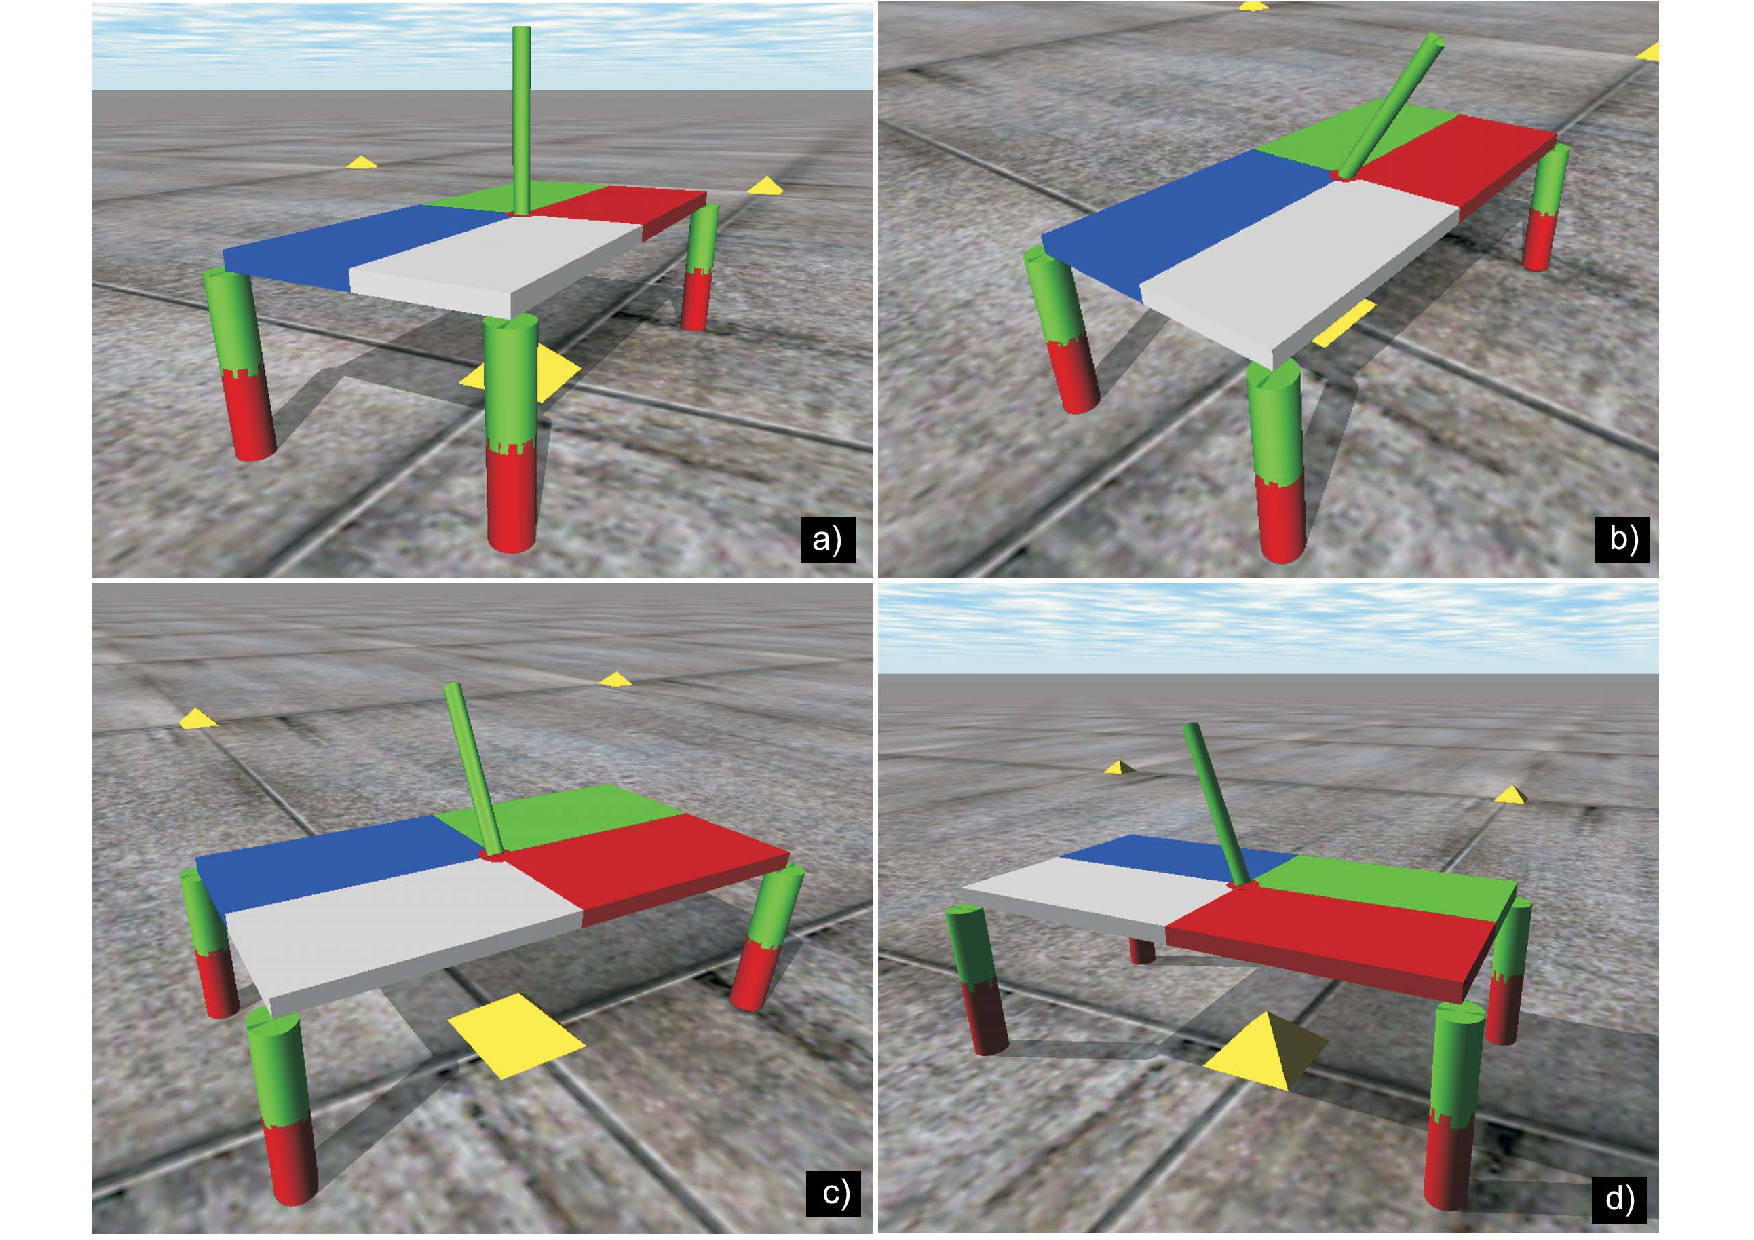
\includegraphics[width=80mm]{./pictures/ODE_simulations.pdf}
	\caption{ODE simulations. a) Initial position b) Test 1. c) Test 2. d) Test 3.}
	\label{fig:ODESimulations}
\end{figure}

Three tests are conducted by changing the initial mass distribution as shown in Table \ref{tab:Simulations}. The first column represents body mass redistribution vector while second and third are final results of tail angles and angular rotation value, respectively. The simulation results are presented in Fig. \ref{fig:ODE graph}. 

Test 1: White and red masses are negligible, the algorithm titled tail in direction $q1=90^{\circ}$. The tail reaches desired position in 7-10 seconds and the final inclination is $q2=32.86^{\circ}$(Fig. \ref{fig:ODESimulations}b). The angular velocity value $\left \| \vec{\omega} \right \|$ goes from $0.14$ to final $0.0025$.

Test 2: Green and blue masses are negligible, the algorithm titled tail in direction $q1=-90^{\circ}$. The final tail inclination is $q2=32.20^{\circ}$(Fig. \ref{fig:ODESimulations}b). The angular velocity value $\left \| \vec{\omega} \right \|$ goes from $0.14$ to final $0.0038$. 

Test 3: The blue mass is negligible, the algorithm titled tail in direction $q1=-26.02^{\circ}$. The final tail inclination is $q2=29.05^{\circ}$(Fig. \ref{fig:ODESimulations}c). The algorithm requires a longer time to minimize $\left \| \vec{\omega} \right \|$ to final $0.0025$(see Table \ref{tab:Simulations2}).

Test 4: Same initial parameters as in Test 3 except the higher gain $K_0$. The desired position is reached faster as expected. The subsequent increase can cause unstable results. 

\begin{table}
	\centering
\begin{tabular}{|c|c|c|c|}
	\hline
$Interation$ & $Q_1$ & $Q_1$  & $\left \| \vec{\omega} \right \|$\\
	\hline
1 & -53.71 & 3.42 & 0.06\\
5 & -33.56 & 9.94 & 0.03\\
10 & -30.72 & 16.24 &  0.025\\
15 & -29.82 & 20.33 & 0.017\\
20 & -29.57 & 22.97 &  0.010\\
25 & -29.09 & 24.83 &  0.008\\
30 & -28.76 & 25.92 &   0.006\\
35 & -28.23 & 27.03 & 0.005\\
40 & -27.40 & 27.74 &0.003\\
45 & -26.34 & 28.40 &  0.0025\\
\hline
\end{tabular}
\caption{Test 3. results}\label{tab:Simulations2}
\end{table}


\begin{figure}
	\centering
	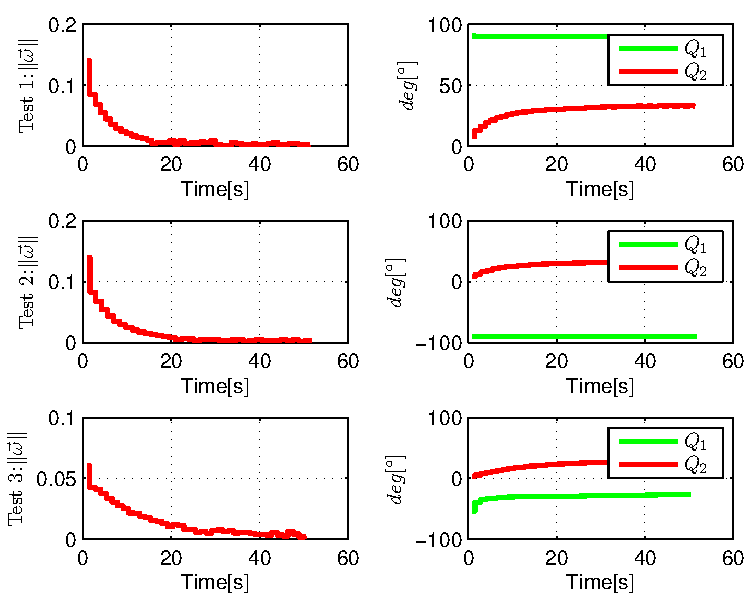
\includegraphics[width=90mm]{./pictures/ODE_graph.pdf}
	\caption{ODE simulations, Test 1-3.}
	\label{fig:ODE graph}
\end{figure}